\documentclass{article}
\usepackage[utf8]{inputenc}
\usepackage{multicol}
\usepackage{amsmath}
\usepackage{subfig}
\usepackage{graphicx}
\usepackage{hyperref}
\usepackage{needspace}

\usepackage[slovak]{babel}
\usepackage[a4paper,top=1.75cm,bottom=1.75cm,left=2.5cm,right=2.5cm,marginparwidth=1.75cm]{geometry}


\title{MVO Projekt - Lineárna Regresia}
\author{Michal Chymo $\frac{1}{2}$, Adam Chrenko $\frac{1}{2}$}
\date{Apríl 2022}

\begin{document}

\maketitle
\section{Popis Problému}
Ľudia sa snažia predikovať budúcnosť odjakživa. S pomocou rôznych nástrojov od kryštálových gúľ cez tarotové karty až po zložité matematické modely a umelú inteligenciu. Jedna z jednoduchších možností, ktorá je ale dosť efektívna je Lineárna regresia. Táto metóda sa snaží nájsť čo najlepšiu čiaru alebo nadrovinu, ktorá čo najlepšie aproximuje už existujúce dáta, za účelom predikcie ďalších dát. 

\section{Matematika}
Na to aby sme vyjadrili minimalizáciu v kompaktnom maticovom zápise použijeme nasledujúci postup
\[\hat{y_i} = \beta_{0} + \beta_{1}x_{i_1} + \beta_{2}x_{i,2} \]
\[min \sum_{i=1}^{m} (\hat{y}_i - y_i)^2\]
Ak si toto rozpíšeme dostávame
\[
min \sum_{i=1}^{m} \left[(\beta_{0} + \beta_{1}x_{i_1} + \beta_{2}x_{i,2}) - y_i\right]^2
\]
Ak nahradíme $\beta_{0} + \beta_{1}x_{i_1} + \beta_{2}x_{i,2}$ pomocou $\mathbf{X_i}\vec{\beta}$ dostaneme prakticky náš výsledok.
\[
min \sum_{i=1}^{m} \left[\vec{\mathbf{X_i}}\vec{\beta} - y_i\right]^2
\]Kde 
\[\mathbf{X} = 
\begin{bmatrix} 
1 & x_{1,1} & x_{1,2} \\ 
1 & x_{2,1} & x_{2,2} \\
\vdots & \vdots & \vdots \\
1 & x_{m,1} & x_{m,2} 
\end{bmatrix}
\qquad\qquad
\Vec{\beta}=
\begin{bmatrix}
\beta_0\\ \beta_1 \\ \beta_2
\end{bmatrix}
\] 

Čo je definícia $L_2^2$ normy. Čiže:

\[
min \|\mathbf{X}\vec{\beta} - y\|_2^2
\]
Ak chceme presné riešenie bety, tak nám stačí dať deriváciu tejto funckie rovnú 0 a vyjadriť betu. Funckia má len jeden extrém a to minimum, čiže aj rovnica kde derivácia sa rovná 0, musí mať jedno riešenie. Derivácia funkcie rovnajúcej sa 0 je:
\[ 2*(\mathbf{X}^T\mathbf{X}\beta) - 2 * (\mathbf{X}^Ty) = 0 \]
Ďalej keď upravíme:
\[ \mathbf{X}^T\mathbf{X}\beta = \mathbf{X}^Ty \]
Vzniká nám sústava 3 rovníc o 3 neznámych a túto sústavu riešime. Všeobecne nám vzniká sústava toľkých rovníc o toľko neznámych koľko rozmerný vstup máme + 1 (V našom prípade je vstup 2-rozmerný a vytvárame rovinu najbližšiu k dátam)

\section{Konštantný krok}
Po nie veľmi zložitom programovaní sa dostávame k výsledkom, že všetky kroky $\geq 1*10^{-6}$ divergujú, tým pádom všetky menšie konvergujú. Otázka je len že ako rýchlo. Ukázalo sa, že krok $10^{-8}$ je zhruba ideálny. Pretože krok $10^{-7}$ konverguje príliš rýchlo, čo vedie k overfitingu (Čo ale technicky nie je problém pri lineárnej regresii, ale je problém pri nelineárnej regresii a iných "Presnejších" metódach).\\
Pri takomto veľkom množstve iterácii štartovací bod prakticky nerobí rozdiel.  Pracujeme na škále 10M iterácii. S najrýchlejšou konvergenciou v zhruba 7.5M iterácii pri kroku s dĺžkou $10^{-7}$.\\ 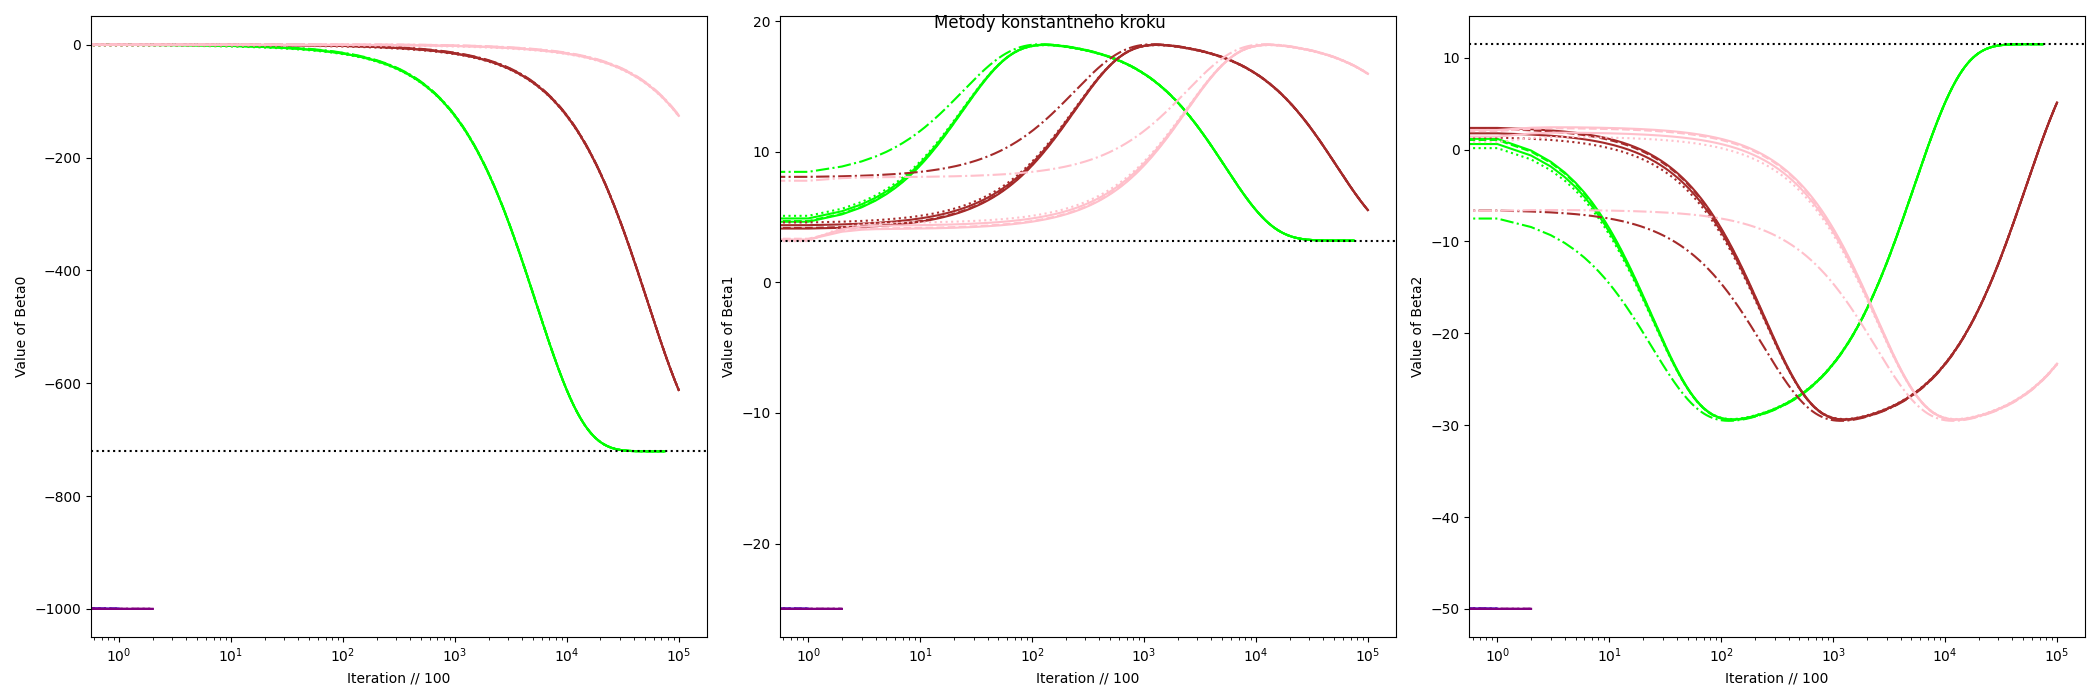
\includegraphics[width=\textwidth]{konstantny_krok.png} \\


\section{Optimálna dĺžka kroku}
Pre túto sekciu sme zvolili metódu, ktorú sme už mali naprogramovanú a odskúšanú z cvičenia. Cauchyho metódu  optimálnym krokom cez metódu zlatého rezu. Keďže táto metóda nepotrebuje žiadne parametre, tak aspoň si skúsime obhájiť voľbu $\epsilon$ - chyba, ktorú sme ochotný akceptovať vo výsledku na $1*10^{-7}$. Toto číslo bolo zvolené, po zistení, že pri $\epsilon \leq 1*10^{-8}$ použité metódy vždy došli až do iteračného limitu. Pretože taká presná konvergencia nie je možná na reálnych dátach(Zo zachovaním generality).\\ Znovu ako je možné vyčítať z grafu, voľba štartovacieho bodu nezaváži signifikantne na počte potrebných iterácii. \\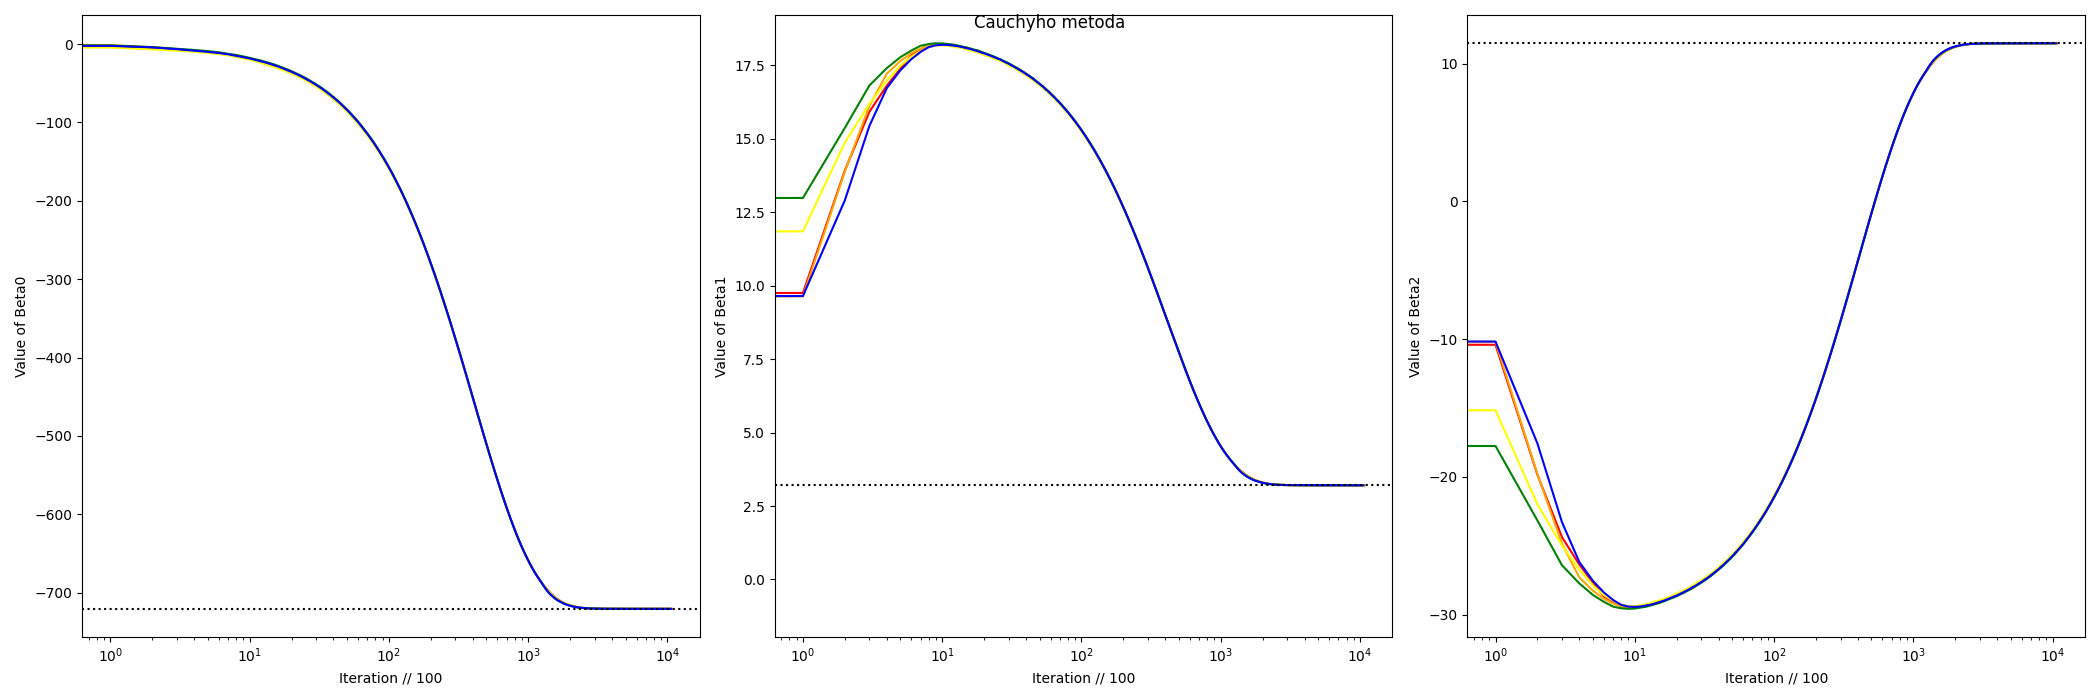
\includegraphics[width=\textwidth]{cauchy.png}  Ale toto môže byť spôsobené aj tým, že sme zvolili štartovacie body dosť blízko pri sebe. Mysleli sme si, že to je dobrý nápad, snažili sme sa zvoliť začiatočné pozície, tak aby metóda mohla mať problém s konvergenciou. Napríklad bod $\left[0,0,0\right]$ mal potenciál byť problematický, pretože jedna z iných metód používa pomery predchádzajúcich bodov ako odhad smeru.\footnote{Chceli sme mať štartovacie body pre všetky metódy rovnaké, pretože v pláne bolo spraviť obrovský interaktívny graf. Toto bohužiaľ nevyšlo keď sme zistili že máme 500MB dát, ktoré tá knižnica proste nevie zobraziť. Takže sme sa museli uspokojiť z takýmito 3x1 stacionárnymi grafmi.}\\


\section{Skoro optimálny krok}
\subsection{Backtracking}
Táto metóda využíva veľmi starý problém(a jeho riešenie), na nájdenie dĺžky krokov blízko optimálnemu bez toho, aby sa musel riešiť celý iný optimalizačný problém o jednej premennej. Na toto využíva prvé Goldsteinove pravidlo resp. jeho aproximáciu a to \[\nabla f(x^k)^T s^k \lambda < f(x^k) + \alpha \nabla f(x^k)^T s^k \lambda  \qquad \alpha \in \left[0,\frac{1}{2}\right]\] ktoré zaručí, že krok bude niekde tesne pod hornou hranicou optimálneho okolia.\\
Z našej skúsenosti táto metóda je najpomalšia zo všetkých testovaných. Áno aj konštantný krok, pretože v tejto metóde každá iterácia trvá omnoho dlhšie ako v konštantnom kroku(cca. 4-6x viac) a zároveň nájdené dĺžky krokov neredukujú počet iterácii dostatočne na to, aby sa kompenzovalo pre dlhší čas strávený na výpočte dĺžky kroku. \\ 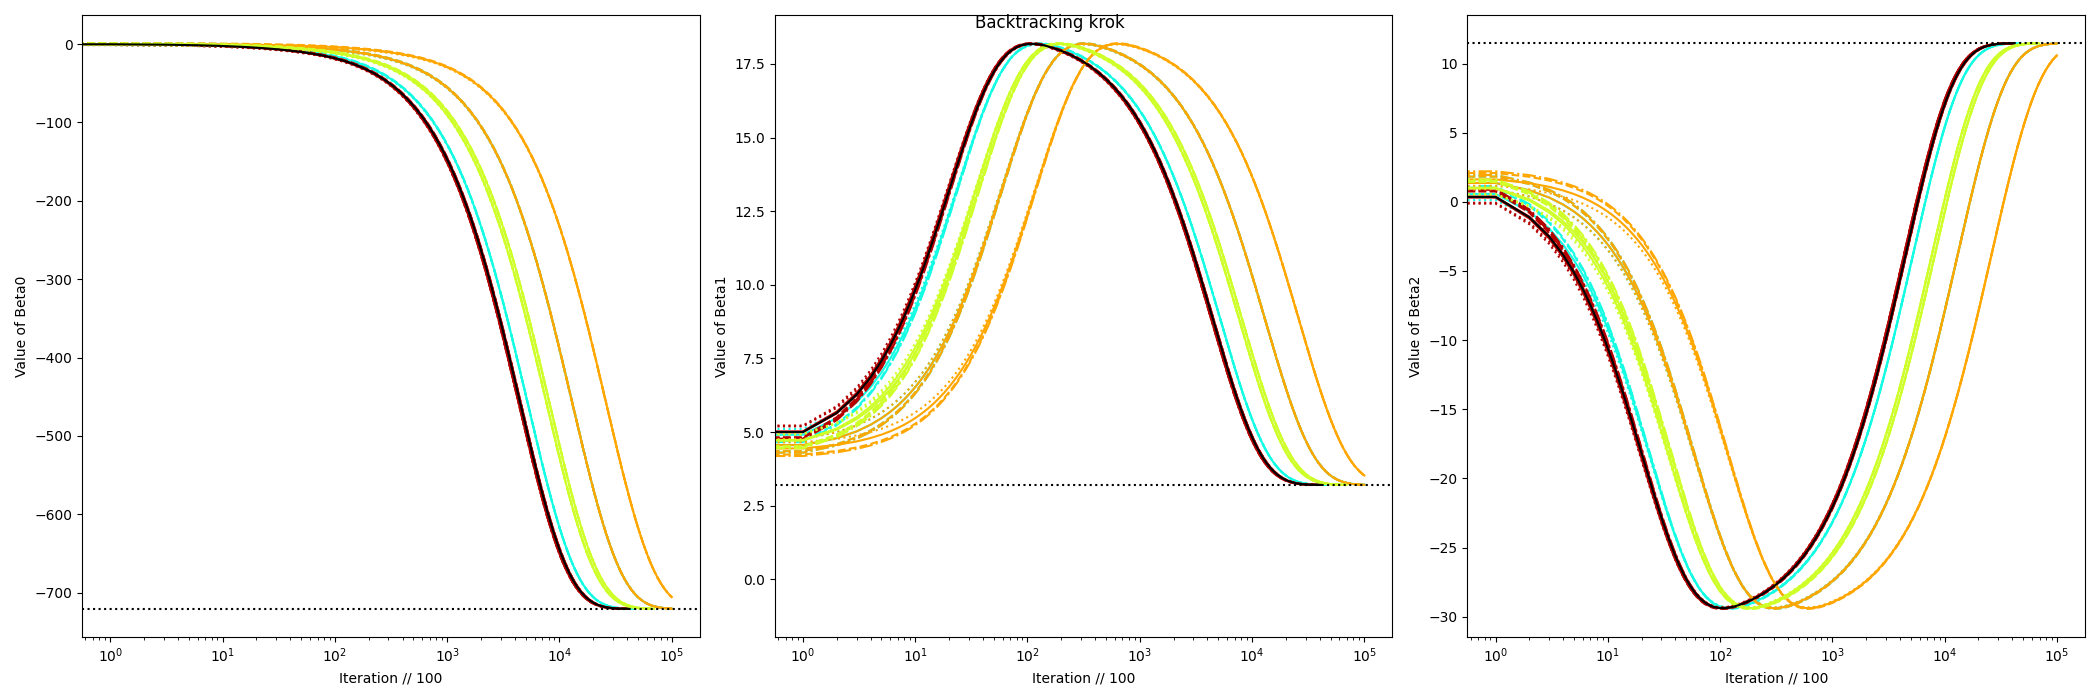
\includegraphics[width=\textwidth]{Backtracking.png}\\
Ako je možné vidieť na grafe, táto metóda s nejakými parametrami ani len nestihla dokonvergovať do správneho riešenia za 10M iterácií. Zároveň oko, ktoré vie na čo sa pozerá si môže všimnúť, že parametre robia dosť veľký rozdiel, skoro 10 násobný.\\
Čierna čiara znázorňuje metódu zo zadanými parametrami a štartovacím bodom v $\left [ 0,0,0\right ]$. Ostatné znázorňujú iné štartovacie body, typ čiary iné parametre. Zadané parametre sú najlepšie z parametrov, ktoré sme použili.
\subsection{Barzilai \& Borwein method - Semi Nadstavba}
Táto metóda je kvázi-newtonovská aj keď sa tak netvári. Podľa whitepaperu v ktorom je definovaná, táto metóda poskytuje dvoj bododovú aproximáciu secantovej rovnice v kvázi-newtonovskej metóde, na ktorej je táto metóda založená\footnote{Normálne kvázi-newtonovské metódy poskytujú len jednobodovú aproximáciu}. Kde dĺžka kroku je definovaná ako 
\[\lambda = \frac{\Delta x^T\Delta x}{\Delta x^T\Delta g} \]
kde 
\[g_k = \nabla f(x_k) \qquad \Delta g = g_k - g_{k-1} \qquad\ \Delta x = x_k - x-{k-1}\]
Táto metóda má extrémne rýchlu konvergenciu, ale chová sa veľmi zvláštne. Skáče všade možne, ale za cenu toho, že používa tento typ kroku, ktorý sa tvári byť "viac než optimálny"(Vychádzam z toho že Cauchyho metóda používa optimálny krok a rovnaký smer, aj tak predsa táto metóda konverguje oveľa rýchlejšie). 
\begin{figure}[h!]
  \caption{Ukradnuté obrázky ilustrujúce ich rozdiely.}
  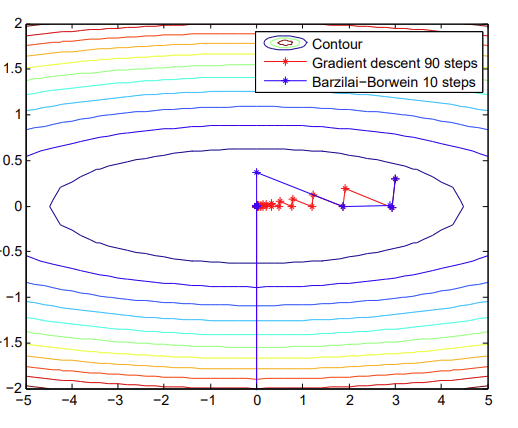
\includegraphics[width=5cm]{GradvsBB.png}
  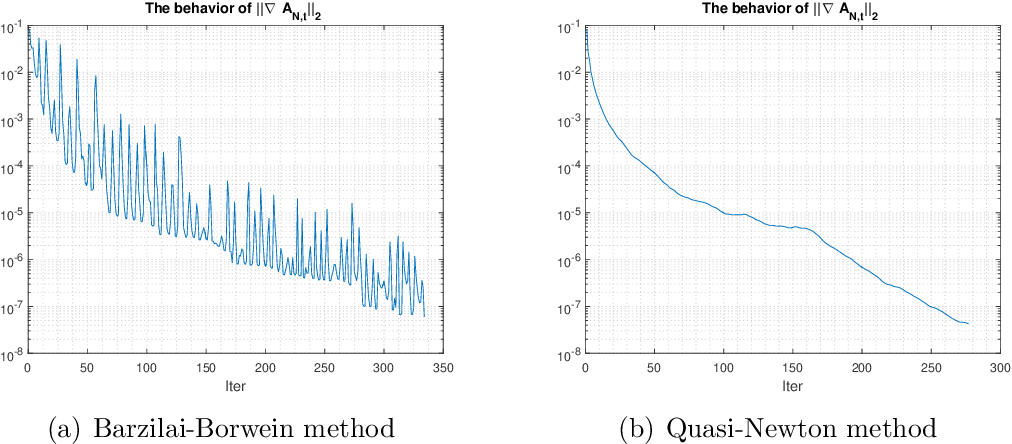
\includegraphics[width=10cm]{Quasi-BB.png}
\end{figure}
Z prvého obrázka je možné vidieť možné vysvetlenie, prečo táto metóda "skáče" aj v našich grafoch. Dĺžka kroku ju vie doviesť do "horších"  miest ako bola v predchádzajúcom stave. Dovolím si povedať, že nie je spádová, aj keď používa záporný gradient ako smer(ktorý spádový je). Priebeh našej optimalizácie touto metódou je zachytený v nasledujúcom grafe.\footnote{Rôzne farby indikujú rôzne štartovacie body}\\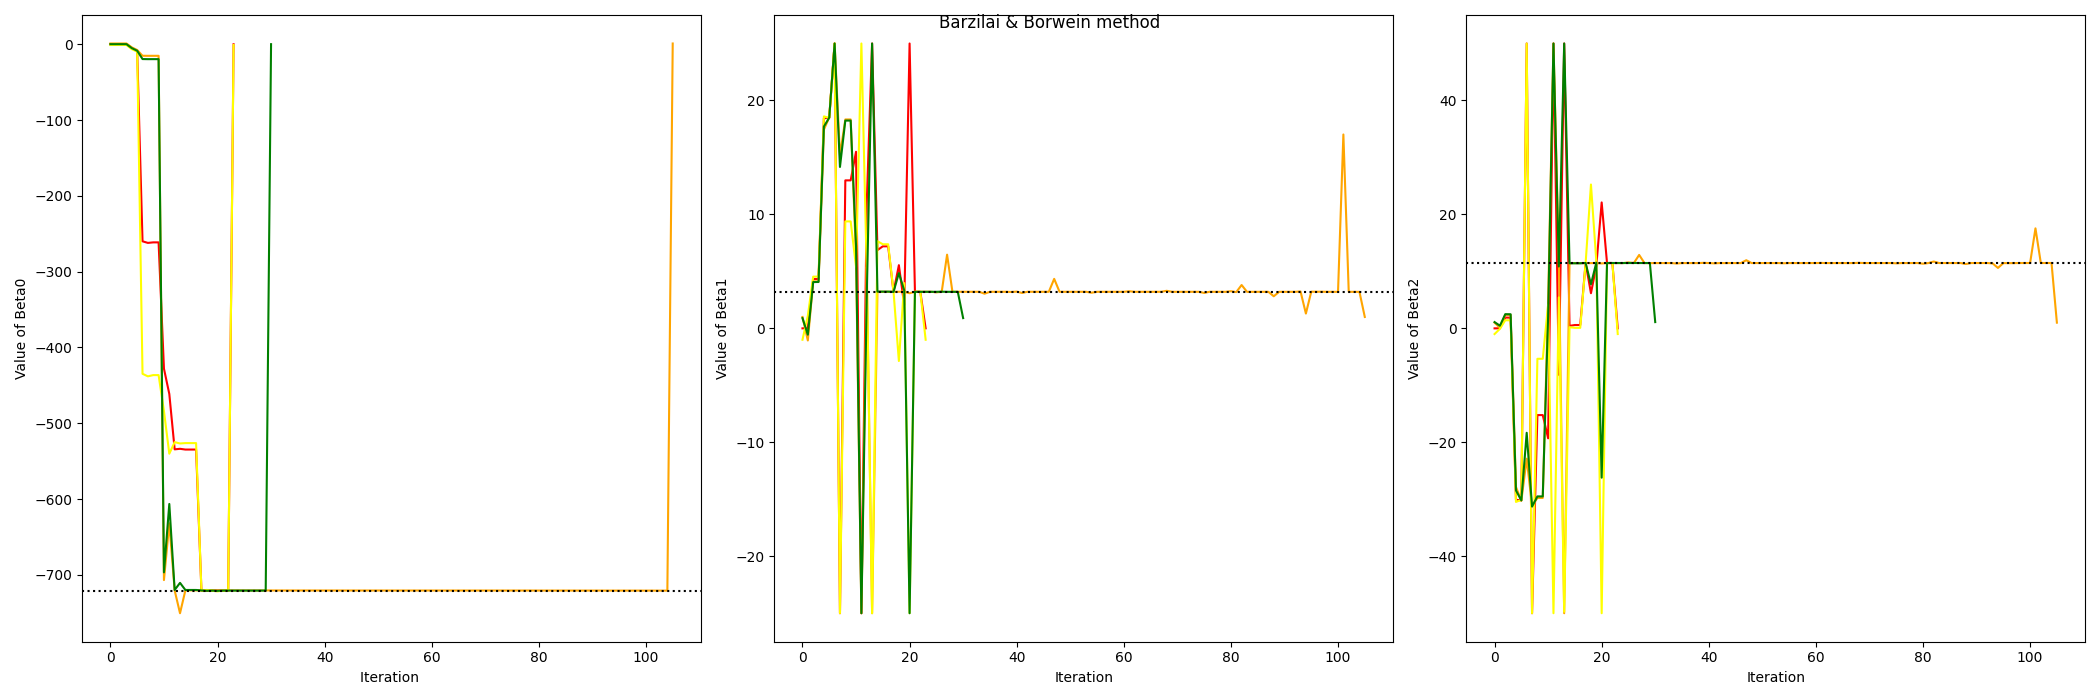
\includegraphics[width=\textwidth]{basil.png}
\section{Odhad na testovacích dátach}
\subsection{Dvojrozmerný vstup (M1,P)}
Hľadali sme najbližšiu rovinu k dátam od roku 1950 po 1980, kde výsledok y(HDP) bol závislý od miery ponuky peňazí $x_1$(M1) a cenového deflátora $x_2$(P). Výsledok bety nám vyšiel po vyriešení sústavy rovníc a aj po hľadaní minima pomocou metód taký istý a to\[ \beta = [-720.71013816,    3.20553725,   11.47092466].\] Koecifient determinácie\footnote{Hovorí nám ako blízko sú dáta k vytvorenej rovine,priamke...(max 1) čím bližšie k 1, tým lepšie} na trénovacích dátach kde sme urobili MNS, nám vyšiel: 0.9977692038451664.
Na dátach od roku 1981 až 1983 nám koeficient determinácie vyšiel: 0.8082238656465313. Pre porovnanie ukážeme aké sú reálne hodnoty HDP od hodnôt vzniknuté na rovine a ich absolútny rozdiel: \\
1.riadok: kvartál, 2. riadok: reálne HDP hodnoty, 3. riadok: predikcia, 4: rozdiel 
\begin{center}
\begin{tabular}{|| c | c | c | c | c | c | c | c | c | c | c | c ||} 
\hline
 1981.1 & 1981.2 & 1981.3 & 1981.4 & 1982.1 & 1982.2 & 1982.3 & 1982.4 & 1983.1 & 1983.2 & 1983.3 & 1983.4 \\  
\hline\hline
 2875.8 & 2918.0 & 3009.3 & 3027.9 & 3026.0 & 3061.2 & 3080.1 & 3109.6 & 3173.8 & 3267.0 & 3346.6 & 3431.7 \\ 
\hline
 2808.1 & 2869.7 & 2933.8 & 2995.3 & 3057.8 & 3097.8 & 3140.1 & 3216.2 & 3294.7 & 3356.4 & 3413.7 & 3460.1 \\
\hline
 67.7 & 48.3 & 75.5 & 32.6 & 31.8 & 36.6 & 60 & 106.6 & 120.9 & 89.4 & 67.1 & 28.4 \\  
\hline
\end{tabular}
\end{center}
suma rozdielov = 764.8
\xpretocmd{\section}{\needspace{6\baselineskip}}{}{}

\subsection{Jednorozmerný vstup (M1)}
Tentoraz hľadáme len priamku keďže vstup máme len 1-rozmerný a to M1(ponuka peňazí). Výsledok bety je:\[ \beta = [-628.79695154,    7.86129104].\] Graf s dátami a spolu s našou MNS priamkou vyzerá:\\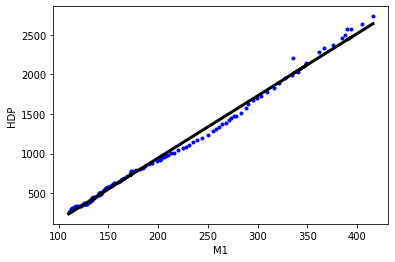
\includegraphics[width=\textwidth]{MNS_1roz_test.png} Jeho koeficient determinácie je (1950 - 1980): 0.994435354959091. Koeficient determinácie tejto priamky na testovacích dátach(1981-1983) je 0.22119671466780022. Ukážme teraz graf testovacích dát spolu s dvomi priamkami, jedna z našej MNS na trénovacích dátach a druhá z MNS na testovacích dátach pre porovnanie: \\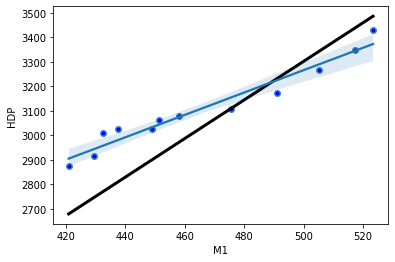
\includegraphics[width=\textwidth]{MNS_test_2.png} Takisto si vypíšme hodnoty a ich rozdiely:\\
1.riadok: kvartál, 2. riadok: reálne HDP hodnoty, 3. riadok: predikcia, 4: rozdiel 
\begin{center}
\begin{tabular}{|| c | c | c | c | c | c | c | c | c | c | c | c ||} 
\hline
 1981.1 & 1981.2 & 1981.3 & 1981.4 & 1982.1 & 1982.2 & 1982.3 & 1982.4 & 1983.1 & 1983.2 & 1983.3 & 1983.4 \\  
\hline\hline
 2875.8 & 2918.0 & 3009.3 & 3027.9 & 3026.0 & 3061.2 & 3080.1 & 3109.6 & 3173.8 & 3267.0 & 3346.6 & 3431.7 \\ 
\hline
 2680.0 & 2746.1 & 2772.0 & 2810.5 & 2899.4 & 2919.0 & 2973.2 & 3110.8 & 3230.3 & 3342.7 & 3437.1 & 3485.8 \\
\hline
 195.8 & 171.9 & 237.3 & 217.4 & 126.6 & 142.2 & 106.9 & 1.2 & 56.5 & 75.7 & 90.5 & 54.1 \\  
\hline
\end{tabular}
\end{center}
suma rozdielov = 1476.1 \\ 
Je vidieť, že vo väčšine hodnôt je predikcia horšia ako pri 2-rozmernom vstupe, ale stále je to dosť dobrá predikcia.
\section{Nadstavba - Regresia pomocou Neurónovej siete}
\subsection{Bleskový úvod}
Neurónové siete alebo takzvané univerzálne odhadovače, sú schopné aproximovať všetky funkcie, ak sú dosť veľké a majú aspoň trošku vhodne zvolené parametere.\\
Neurónová sieť sa skladá z perceptronov, tieto základné stavebné jednotky sú veľmi jednoduché. Vieme si ich predstaviť ako lineárnu funkciu s predpisom $f(x):  mx + b$ a takzvanou aktivačnou funkciou. Toto môže byť prakticky hocijaká nelineárna funkcia(Často používané sú tzv. Rectified linear - $f(x): \frac{x | x >0}{0 | x \leq 0}$ a hyperbolický tangens).
Ak skombinujeme dostatok týchto perceptronov, vieme konštruovať všetky nelineárne funkcie.
Ale tieto perceptrony musia byť natrénované. Proces trénovania siete je podobný ako proces lineárnej regresie.
\begin{enumerate}
    \item Zvolíme náhodný štartovací bod.
    \item Preženieme dáta touto sieťou.
    \item Vypočítame funkciu straty. V našom prípade - $(\hat{y} - y)^2$
    \item Re-distribuujeme spätne túto chybu, využitím parciálnych derivácii a kto vie čoho ešte, toto knižnica robí za nás.
    \item Toto nám zmení m,b v našich perceptronoch. Tým pádom vedia trošku lepšie povedať čo sa deje.
    \item Opakuj $[2-6]$ až do pokiaľ strata nie je dostatočne malá alebo dosiahne bod kedy už sa nezlepšuje.
\end{enumerate}
\subsection{Naša sieť a jej výsledky}
Ako našu sieť sme si zvolili plne spojenú 4 stupňovú sieť. Ako optimalizér sme použili najštandardnejší optimalizér Adam\footnote{Toto je možné robiť aj pomocou metód, ktoré sme mali na prednáške. Často používaná je Stochastická Gradientná Metóda(SGD), a Nesterovo Urýchlenie(AGD). Ale tieto metódy sú objektívne horšie ako tá, ktorú sme použili}. Po zhruba 4500 iteráciách(čo zabralo menej času ako optimalizácia cez backtracking), sme sa dostali do bodu 6, kde sa naša strata začala zvyšovať.\\
Po predikovaní dát v testovacom súbore sa dostávame na koeficient determinácie 0.92, čo je omnoho lepšie ako koeficienty, ktoré sme dostali s našou lineárnou regresiou(0.8). Zaujimave je, že lineárna regresia má vyšší koeficient determinácie na trénovacom sete dát ako táto sie,ť ale v predikcii má o dosť horší, z čoho vyplýva, že lineárna regresia overfituje, čo som si nebol vedomý, že je možné.
3D graf reálnych dát, regresnej priamky a dát predikovaných sieťou je na \href{https://adam-213.github.io/MVO2022/}{githube}.


\end{document}
